\section{Experimentación General}


\subsection{Comparando con el Exacto}

\quad Vamos a comparar todas nuestras implementaciones y a calcular las distancias con respecto al algoritmo exacto. Debido al costo del exacto se realizaron tests de 5 nodos a 17 con 50 repeticiones para cada cantidad. Definimos distancia como la diferencia entre el resultado exacto y el de la heurística correspondiente. 


\quad Comparamos primero con grafos generados aleatoriamente, luego con grafos estrellas no uniformes y grafos \textit{web}.


\begin{figure}[H]
	\centering
	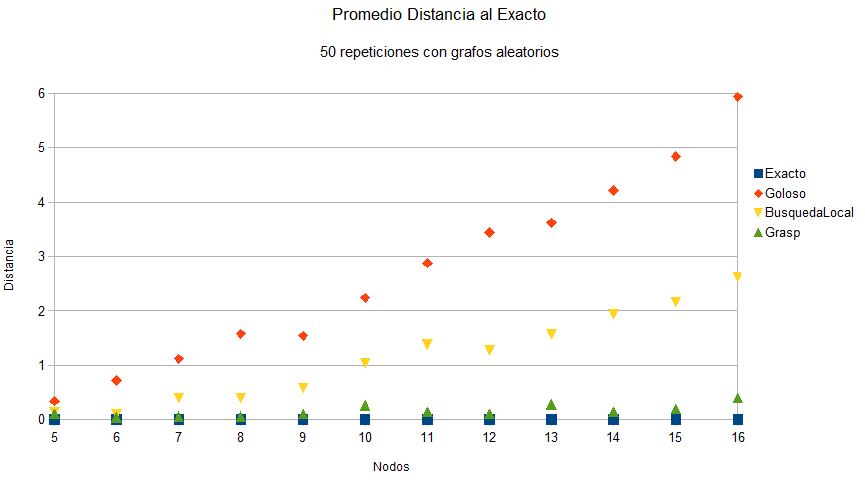
\includegraphics[scale=0.6]{distancia-Azar.png}
\end{figure}


%\begin{figure}[H]
%	\centering
%	\includegraphics[scale=0.8]{distancia-Estrella.png}
%\end{figure}
%
%\begin{figure}[H]
%	\centering
%	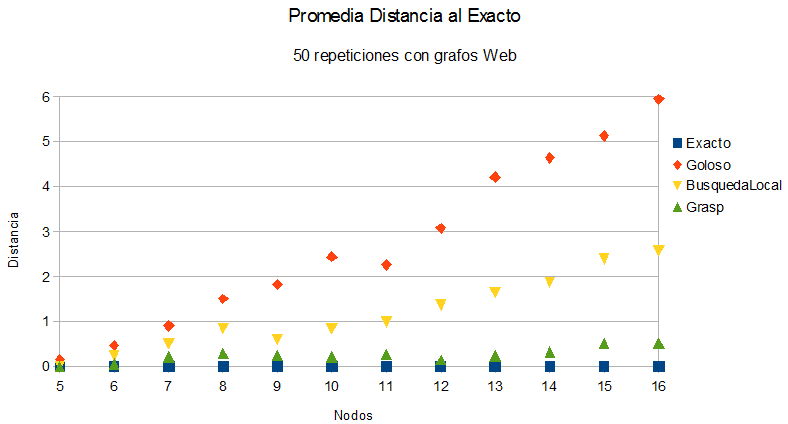
\includegraphics[scale=0.8]{distancia-Web.png}
%\end{figure}

\quad



\subsection{Comparando con Grasp}

\quad Dejando de lado el algoritmo exacto, podemos experimentar con una mayor cantidad de nodos. Comparamos la heuristica golosa, la búsqueda local y GRASP

\subsubsection{Efectividad}

\begin{figure}[H]
	\centering
	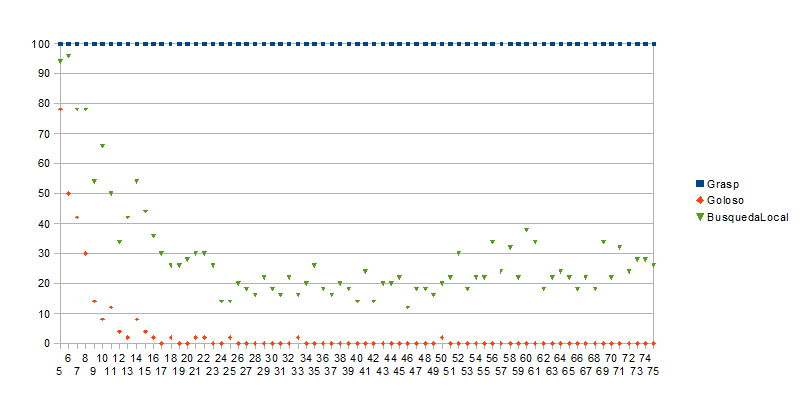
\includegraphics[scale=0.8]{efectividad-vs-grasp.png}
\caption{Comparación de efectividad contra Grasp}
\end{figure}

\quad Podemos ver como a partir de cierto punto, la heurística golosa no es para nada efectiva (según el criterio anteriormente mencionado). En cambio, la búsqueda local se \textit{estanca} entre el 10 \%  y 40 \%  de efectividad.

\subsubsection{Costo}

\begin{figure}[H]		
	\centering
	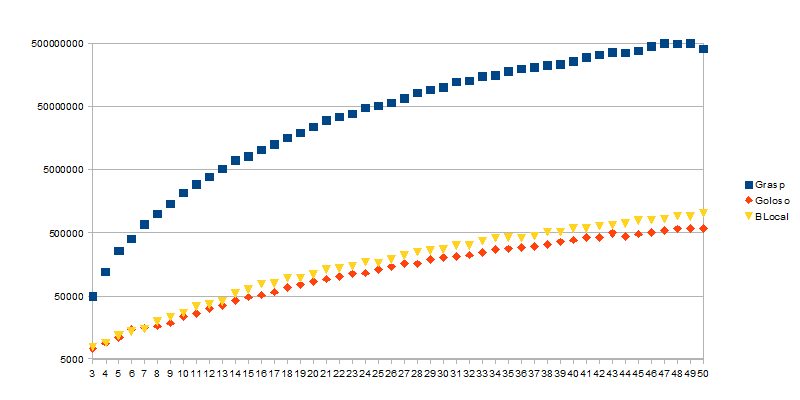
\includegraphics[scale=0.8]{timing-vs-grasp.png}
\caption{Costo temporal de las heurísticas, en escala logaritmica, contra Grasp}
\end{figure}

\quad En este gráfico podemos observar como GRASP a pesar de obtener resultados mucho mejores que las otras heuristicas, consume mucho más tiempo de procesamiento.

\quad Si bien la búsqueda local cuesta apenas más que la golosa, en comparación con GRASP, se obtiene muchos mejores resultados.
